% ============================================================================
% The Consciousness Series
% Complete Collected Volume
% ============================================================================

\documentclass[12pt,a4paper,openany]{book}

\usepackage[utf8]{inputenc}
\usepackage[T1]{fontenc}
\usepackage{amsmath,amssymb,amsfonts,amsthm}
\usepackage{graphicx}
\usepackage[hidelinks]{hyperref}
\usepackage{pdfpages}
\usepackage{geometry}
\usepackage{fancyhdr}
\usepackage{array}
\newcolumntype{P}[1]{>{\raggedright\arraybackslash}p{#1}}
\usepackage{booktabs}
\usepackage{xcolor}
\usepackage{caption}
\usepackage{float}

\geometry{a4paper, margin=1in, headheight=28pt}

\pagestyle{fancy}
\fancyhf{}
\fancyhead[LE,RO]{\thepage}
\fancyhead[RE]{\textit{The Consciousness Series}}
\fancyhead[LO]{\textit{\leftmark}}
\renewcommand{\headrulewidth}{0.4pt}

\title{
  \vspace{-2cm}
  {\Huge\textbf{The Consciousness Series}}\\[1cm]
  {\Large\textit{From Source Formation to Geometry, Gravity,\\
  and the Structural Horizon of Self-Description}}\\[2cm]
  {\large Complete Collected Volume}\\[0.5cm]
  {\normalsize Foundation Trilogy \textperiodcentered{} Consciousness Trilogy}
}

\author{
  \textbf{Sidong Liu, PhD}\\[0.5em]
  iBioStratix Ltd\\[0.3em]
  \texttt{sidongliu@hotmail.com}
}

\date{April 2026}

\hypersetup{
  pdftitle={The Consciousness Series},
  pdfauthor={Sidong Liu},
  pdfsubject={Zenodo upload edition of Foundations I--III and Papers I--III},
  pdfkeywords={open quantum systems, quantum dynamical semigroups, von Neumann algebras, Type III1 factors, modular theory, same-root structure, shared manifestation, source-level feedback, geometry-modular inseparability, linearized gravity, self-description}
}

\begin{document}
\emergencystretch=2em
\raggedbottom
\hbadness=5000
\vbadness=5000

\frontmatter
\maketitle

\newpage
\thispagestyle{empty}
\vspace*{\fill}
\begin{center}
\textbf{Publication Record}\\[2em]
{\small
\begin{tabular}{P{4.1cm}P{4.5cm}P{5.6cm}}
\textbf{Consciousness Series} & DOI: 10.5281/zenodo.19643449 & Complete six-paper collection \\[1em]
\multicolumn{3}{l}{\textbf{Part~I --- Foundation Trilogy}} \\[0.5em]
Foundation Trilogy & DOI: 10.5281/zenodo.19642398 & Foundations I--III collection \\
Foundation I v2 & DOI: 10.5281/zenodo.19627786 & From Source to Manifestation \\
Foundation II & DOI: 10.5281/zenodo.19641372 & Shared Manifestation \\
Foundation III & DOI: 10.5281/zenodo.19642189 & The Perfuming Loop \\[0.8em]
\multicolumn{3}{l}{\textbf{Part~II --- Consciousness Trilogy}} \\[0.5em]
Consciousness Trilogy & DOI: 10.5281/zenodo.19608174 & Papers I--III collection \\
Paper I & DOI: 10.5281/zenodo.19607387 & Geometry and Modular Flow \\
Paper II & DOI: 10.5281/zenodo.19607543 & Higher-Dimensional Consistency \\
Paper III & DOI: 10.5281/zenodo.19607724 & Structural Horizon of Self-Description \\
\end{tabular}
}
\\[3em]
\textit{This collected volume compiles previously published works\\
for archival and reference purposes. Foundation~I appears here in its
current v2 interface-harmonized text.}
\\[2em]
\copyright{} 2026 Sidong Liu. All rights reserved.
\end{center}
\vspace*{\fill}

\chapter*{Abstract}
\addcontentsline{toc}{chapter}{Abstract}

This volume collects the six papers comprising the
\emph{Consciousness Series}---a programme that investigates how
source-side open-system structure, manifest carriers, geometry,
gravitational consistency, and the structural limits of self-description
fit into a single operator-algebraic chain.

The programme is organised in two parts:

\begin{enumerate}
\item \textbf{Part~I: Foundation Trilogy} (Foundations~I--III).
  The Foundation papers develop the source-side scaffolding of the
  programme. They argue that:
  (a)~a single Type~III$_1$ source datum can, under named conditional
  inputs, reach an admissible manifest carrier;
  (b)~multiple source chains can admit a conditional shared manifest
  sector without any tensor-product assumption; and
  (c)~a manifest calibration signal can be lifted back to a conditional
  one-step source-level feedback loop by exact semigroup composition.

\item \textbf{Part~II: Consciousness Trilogy} (Papers~I--III).
  The Consciousness papers analyze what follows once such an admissible
  manifest sector is available. They argue that:
  (a)~geometry and modular flow are structurally inseparable in the
  stated Type~III$_1$ regime;
  (b)~higher-dimensional consistency of the modular datum yields the
  linearized Einstein equation in the CHM small-ball regime; and
  (c)~finite self-description leaves a quantitative local minimax
  relative-entropy deficit floor.
\end{enumerate}

Taken together, the two parts establish a six-paper programme: source
formation, shared stabilization, one-step feedback, geometry--modular
inseparability, gravitational consistency, and a final quantitative
horizon on self-description.

\bigskip
\noindent\textbf{Keywords}: open quantum systems, quantum dynamical
semigroups, von Neumann algebras, Type~III$_1$ factors, modular theory,
same-root structure, geometry--modular inseparability, linearized
gravity, self-description

\tableofcontents

\mainmatter

\part{Foundation Trilogy: Source Formation, Shared Manifestation, and Feedback}

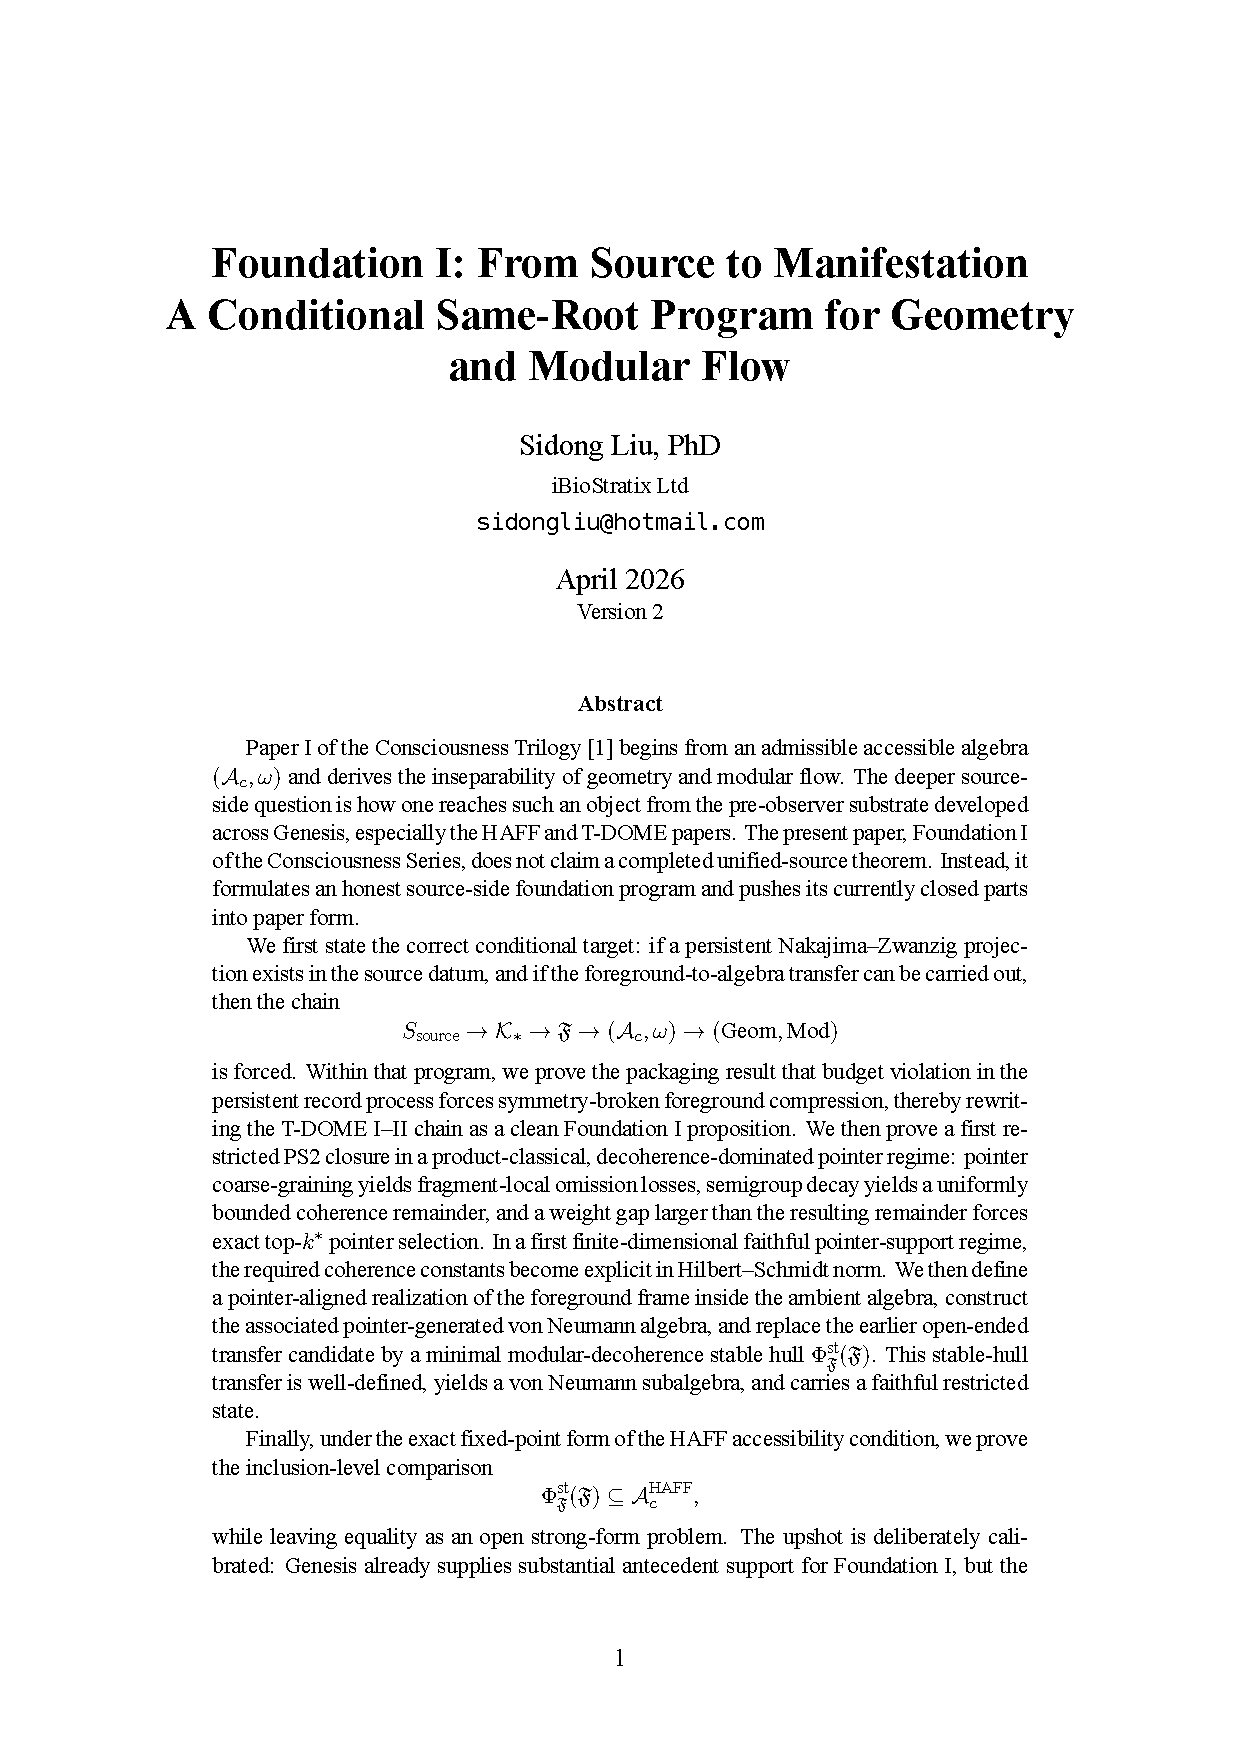
\includepdf[
  pages=-,
  pagecommand={\thispagestyle{empty}},
  addtotoc={1,chapter,1,{Foundation I: From Source to Manifestation},chap:foundationI}
]{../Zenodo/Foundation_I_From_Source_to_Manifestation_Zenodo_v2.pdf}

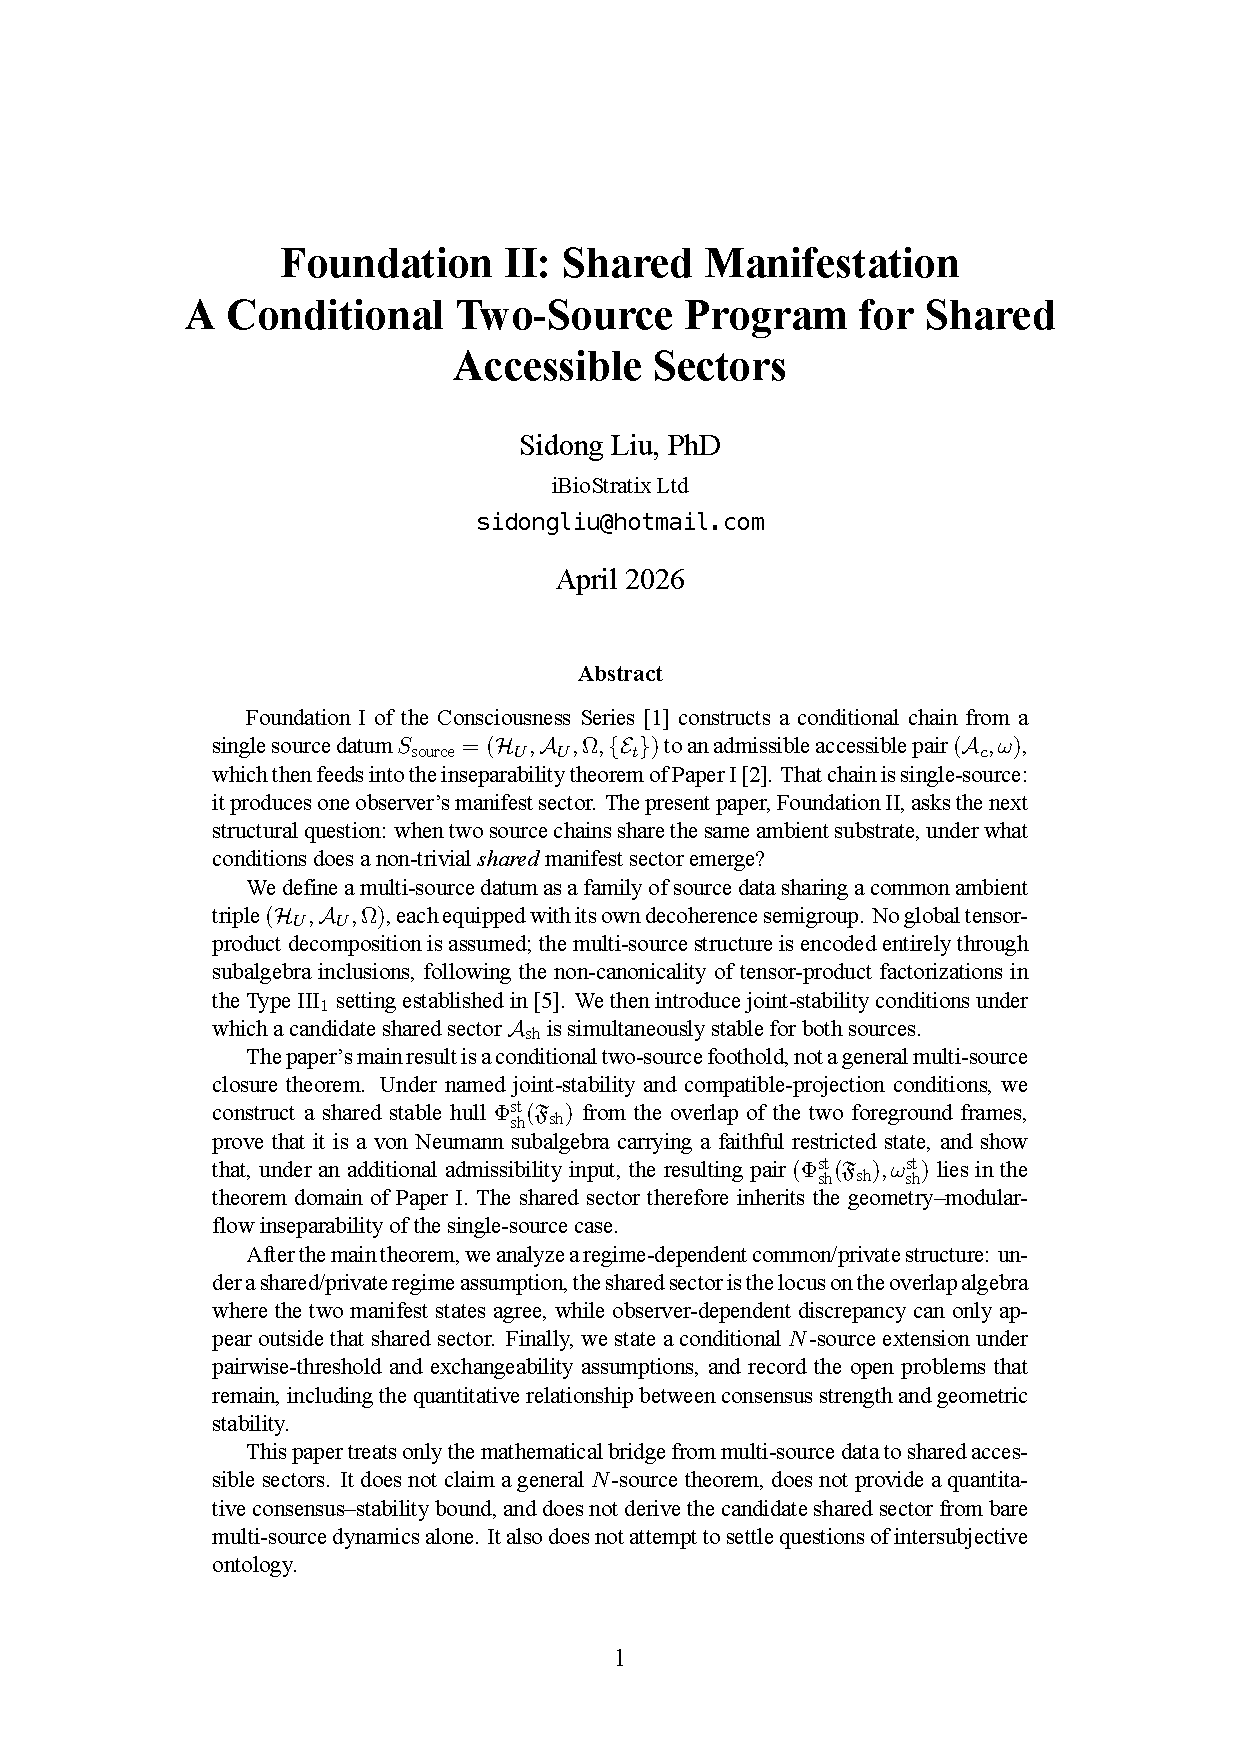
\includepdf[
  pages=-,
  pagecommand={\thispagestyle{empty}},
  addtotoc={1,chapter,1,{Foundation II: Shared Manifestation},chap:foundationII}
]{../Zenodo/Foundation_II_Shared_Manifestation_Zenodo.pdf}

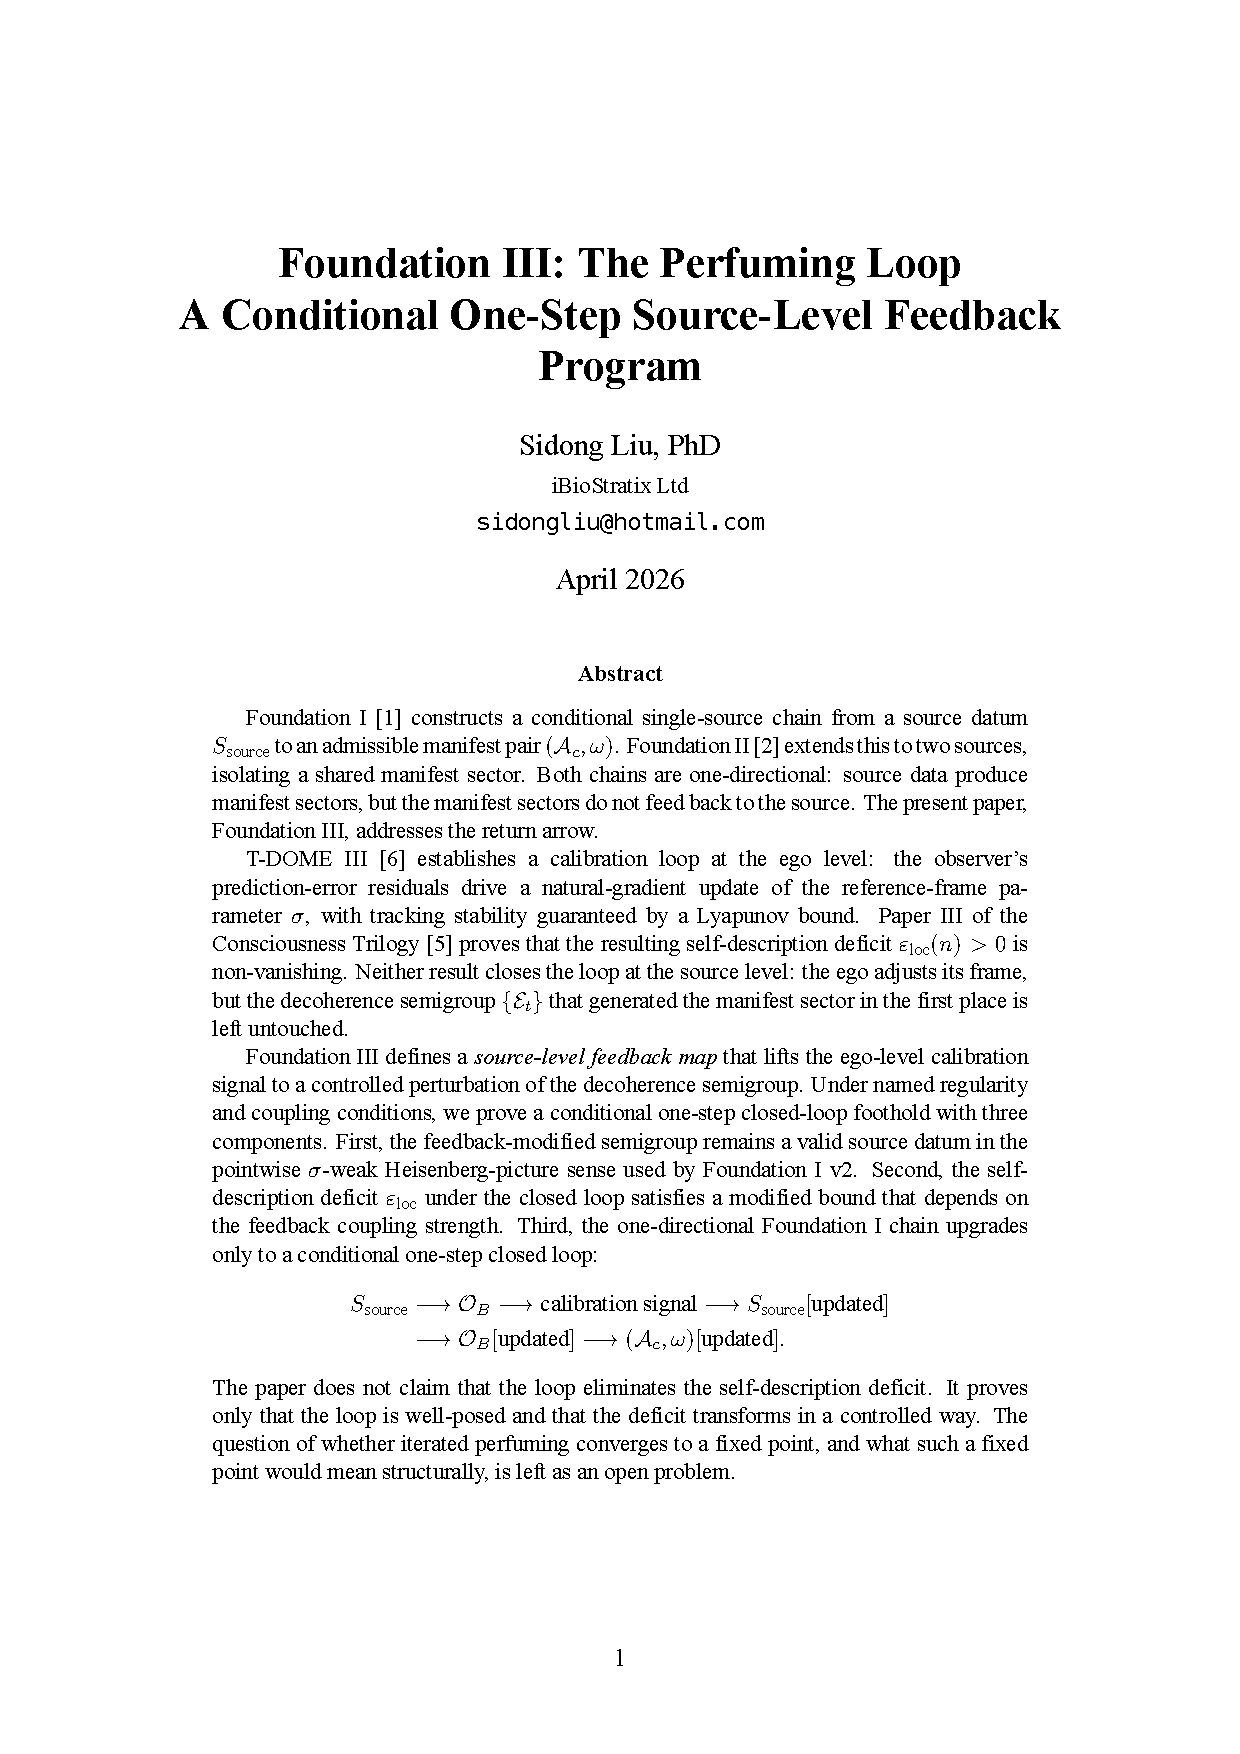
\includepdf[
  pages=-,
  pagecommand={\thispagestyle{empty}},
  addtotoc={1,chapter,1,{Foundation III: The Perfuming Loop},chap:foundationIII}
]{../Zenodo/Foundation_III_The_Perfuming_Loop_Zenodo.pdf}

\part{Consciousness Trilogy: Geometry, Gravity, and the Structural Horizon of Self-Description}

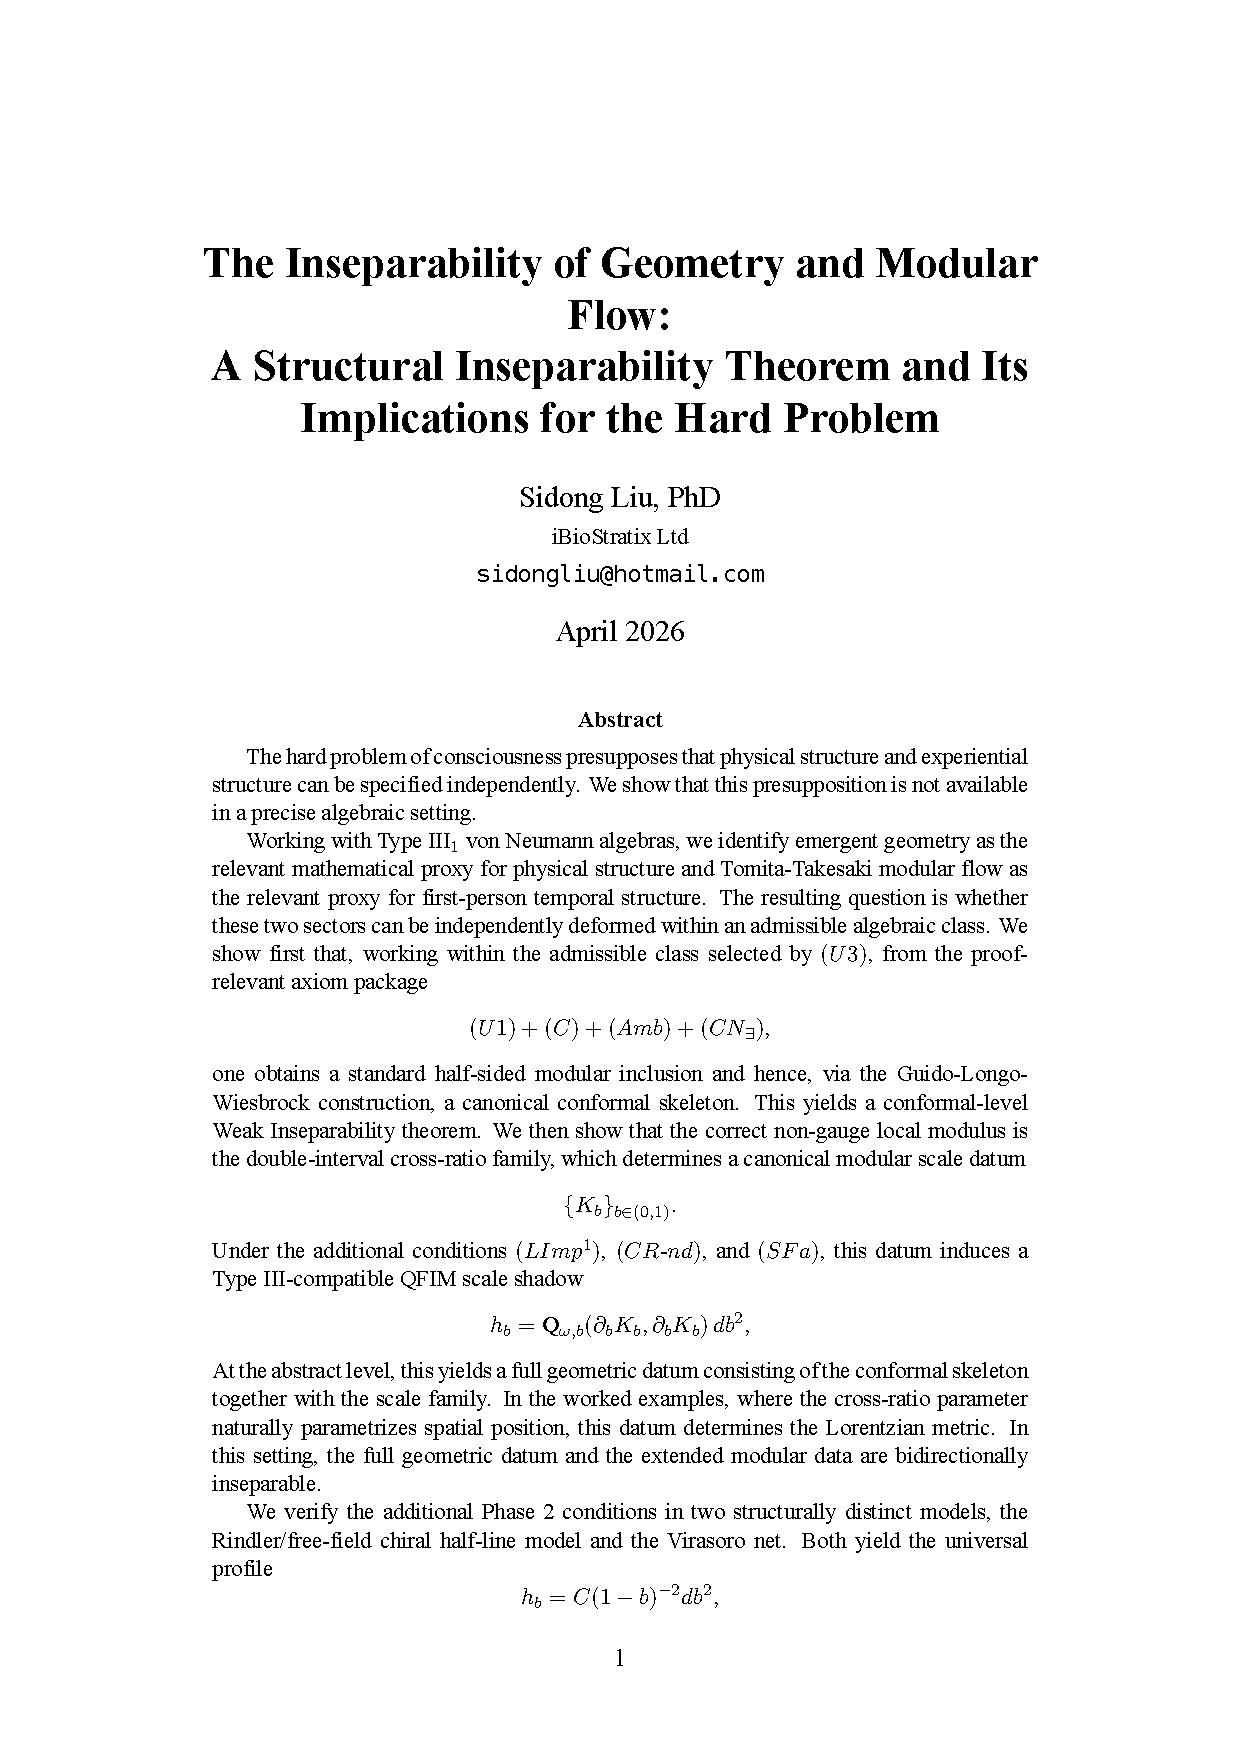
\includepdf[
  pages=-,
  pagecommand={\thispagestyle{empty}},
  addtotoc={1,chapter,1,{Paper I: The Inseparability of Geometry and Modular Flow},chap:paperI}
]{../Zenodo/Paper_I_The_Inseparability_of_Geometry_and_Modular_Flow_Zenodo.pdf}

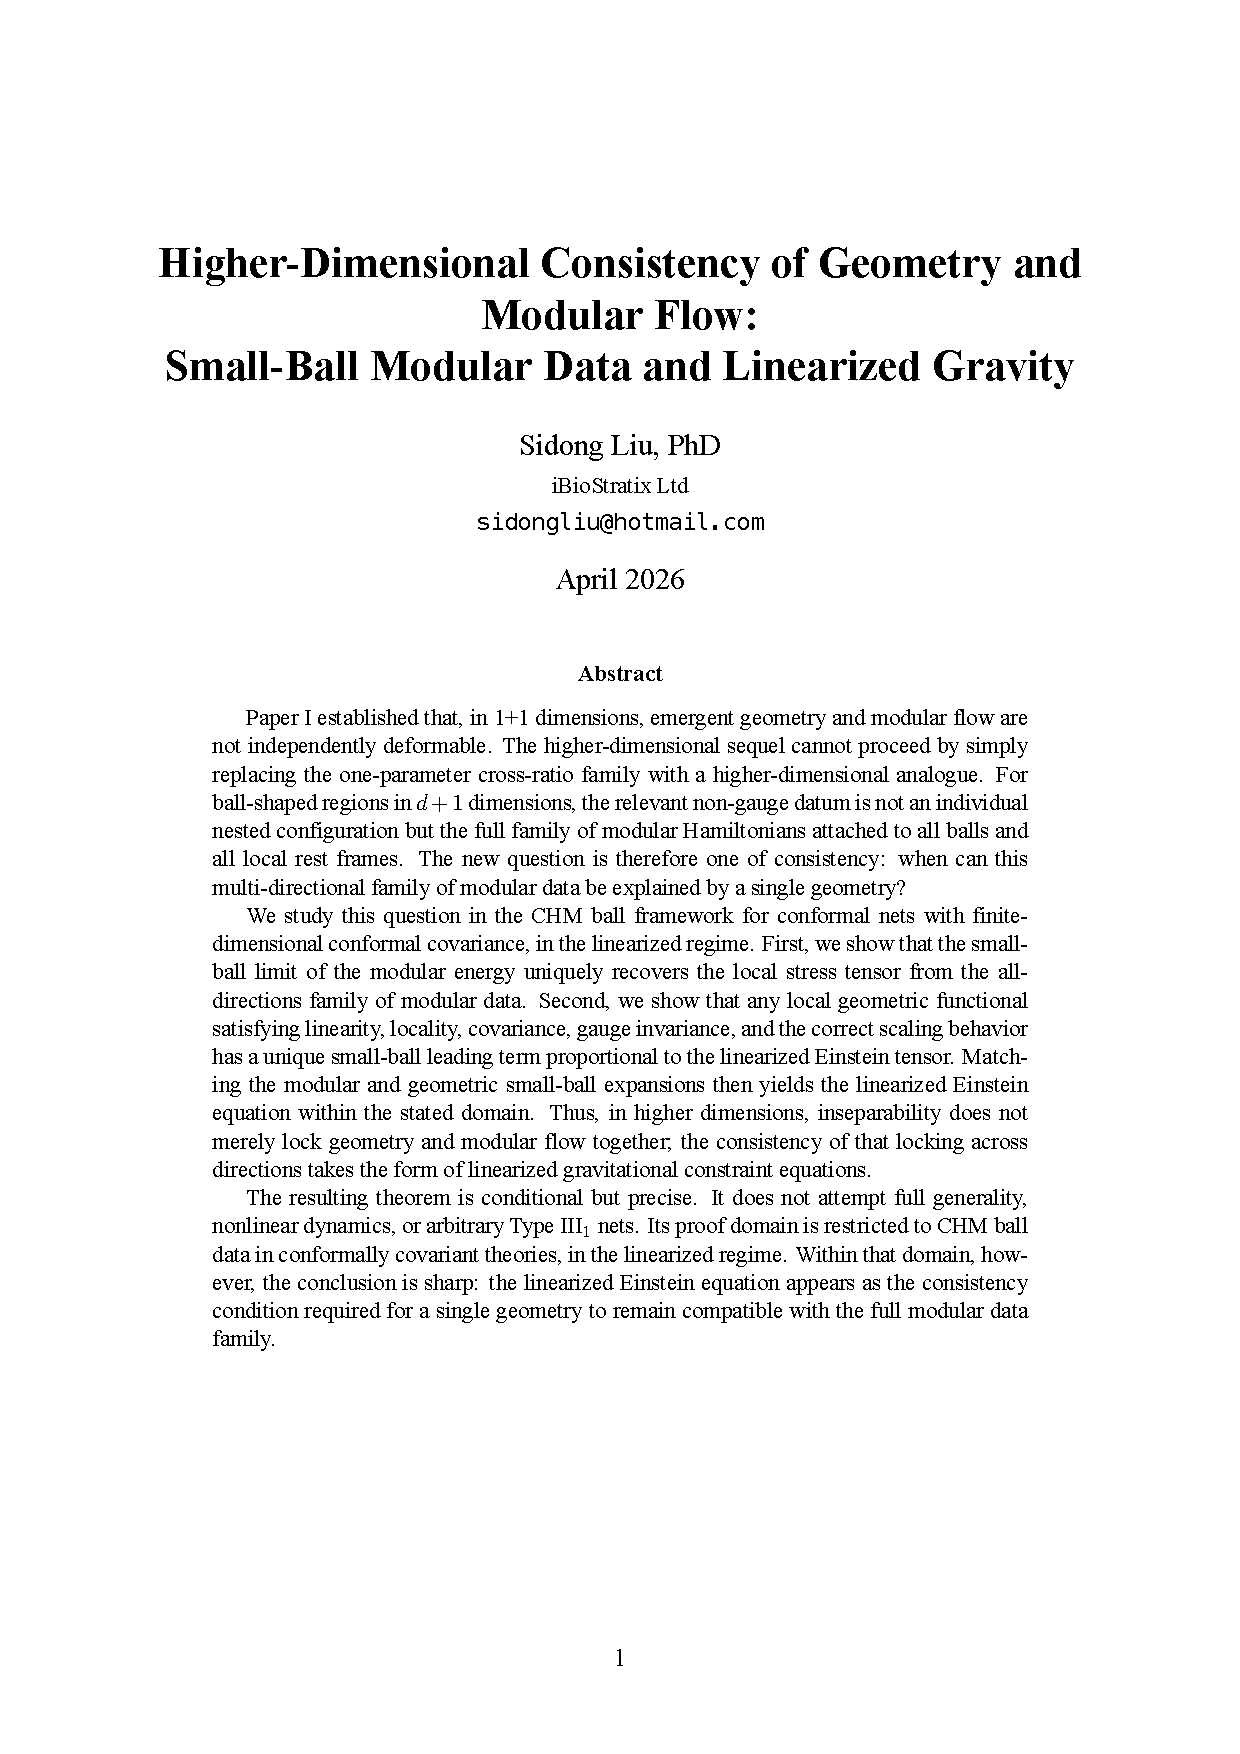
\includepdf[
  pages=-,
  pagecommand={\thispagestyle{empty}},
  addtotoc={1,chapter,1,{Paper II: Higher-Dimensional Consistency of Geometry and Modular Flow},chap:paperII}
]{../Zenodo/Paper_II_Higher_Dimensional_Consistency_Zenodo.pdf}

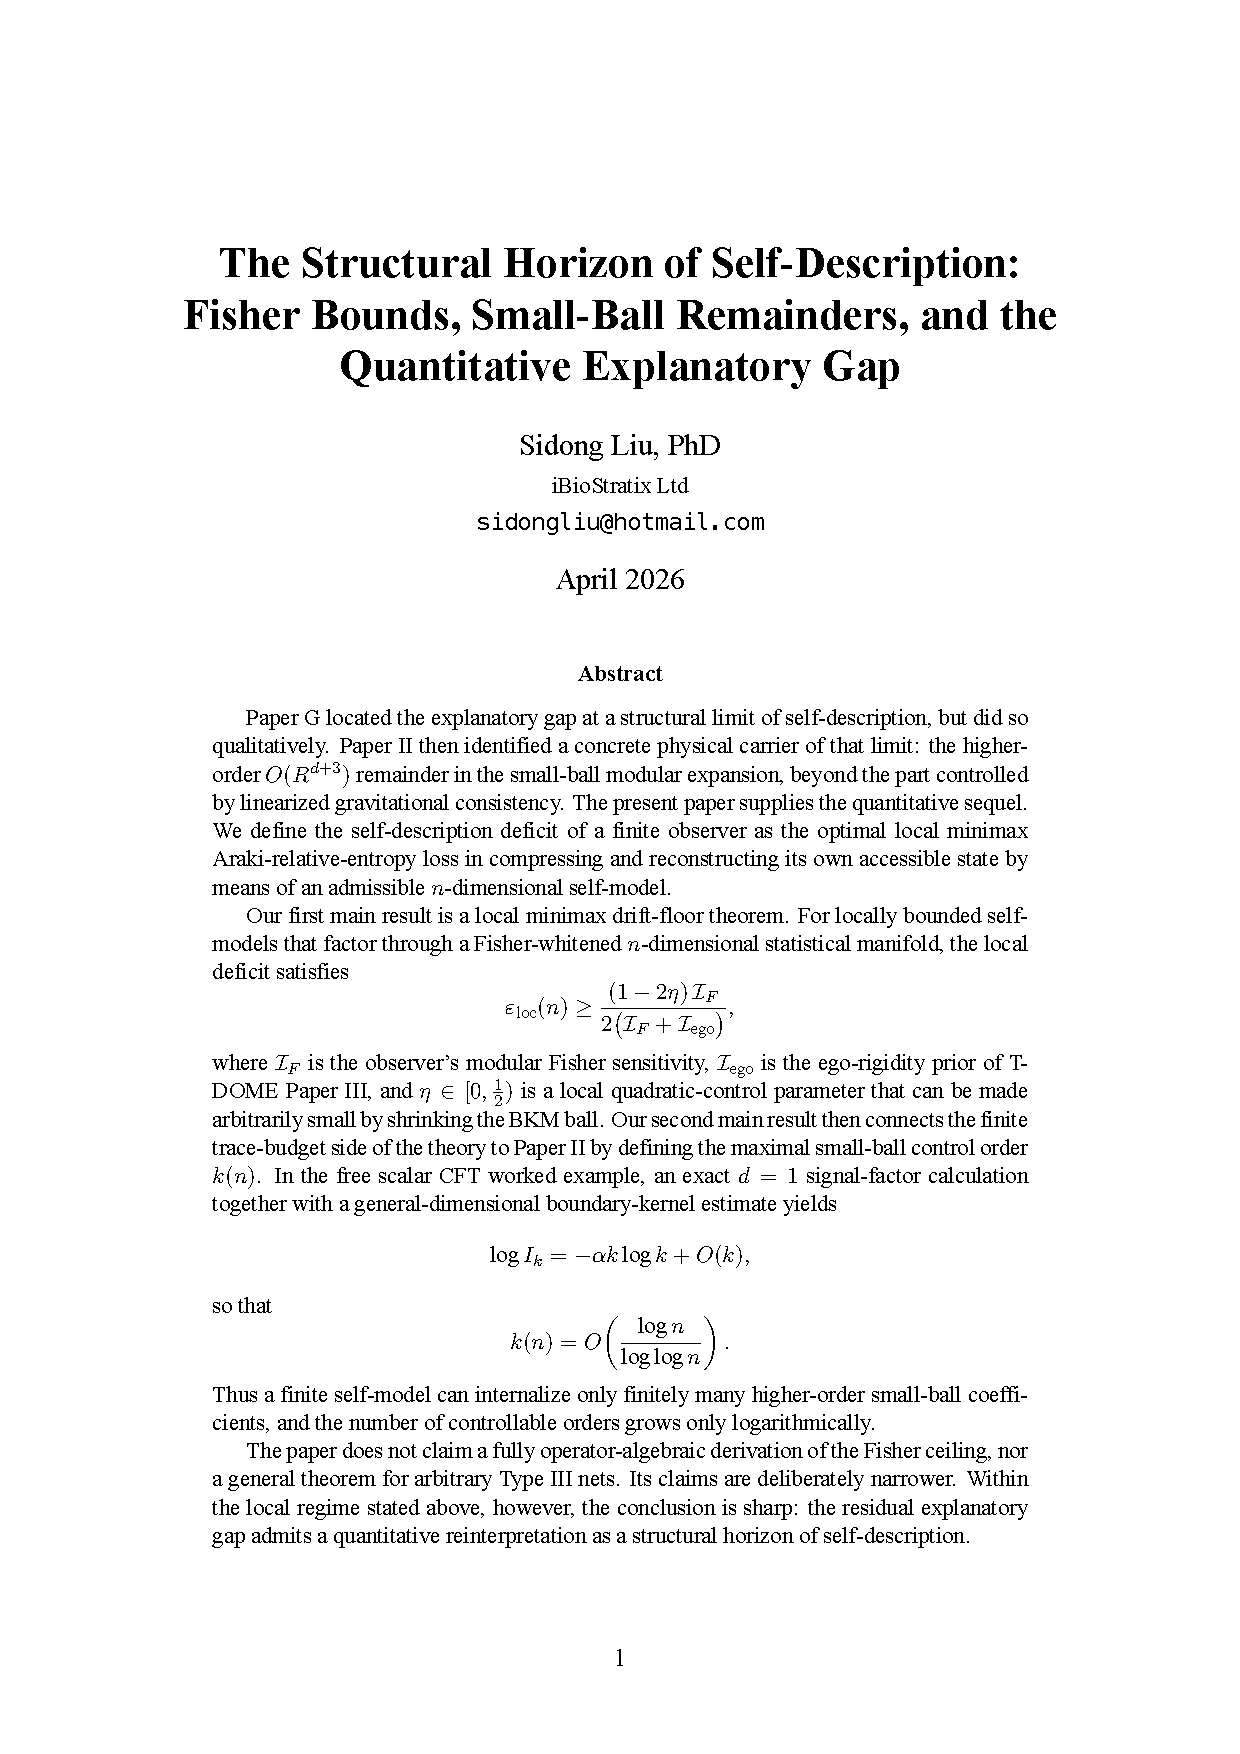
\includepdf[
  pages=-,
  pagecommand={\thispagestyle{empty}},
  addtotoc={1,chapter,1,{Paper III: The Structural Horizon of Self-Description},chap:paperIII}
]{../Zenodo/Paper_III_The_Structural_Horizon_of_Self_Description_Zenodo.pdf}

\end{document}
